\documentclass[../../main.tex]{subfiles}

\begin{document}

\subsubsection*{Auswertung Fragen zum Unternehmensumfeld}
\addcontentsline{toc}{subsubsection}{Auswertung Fragen zum Unternehmensumfeld}

\subparagraph*{Frage: Der Firmencomputer ist sicher}\mbox{}
\begin{figure}[H]
\centering
\framebox[\textwidth]{\scriptsize 0 = Trifft überhaupt nicht zu $\vert$ 100 = Trifft voll zu ($n: 255$, $\bar{x}: 78.42$, $\sigma: 20.49$)}
\framebox[\textwidth]{\scalebox{0.9}{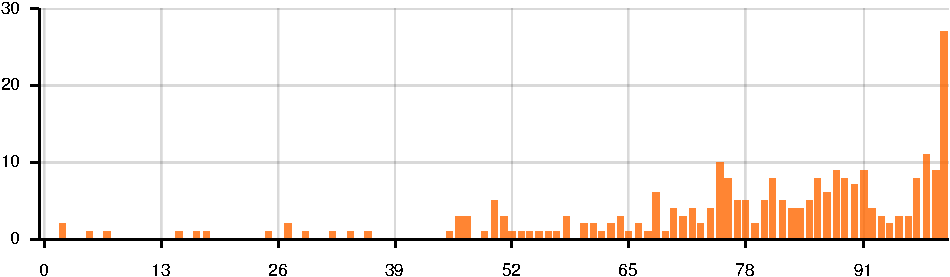
\includegraphics{figures/esurvey/c_com_u17_companydev}}}
\caption{Auswertung Frage U17}
\label{U17}
\end{figure}

\subparagraph*{Frage: Bin selber Verantworlich für Schutz von Firmencomputer}\mbox{}
\begin{figure}[H]
\centering
\framebox[\textwidth]{\scriptsize 0 = Trifft überhaupt nicht zu $\vert$ 100 = Trifft voll zu ($n: 255$, $\bar{x}: 69.49$, $\sigma: 28.03$)}
\framebox[\textwidth]{\scalebox{0.9}{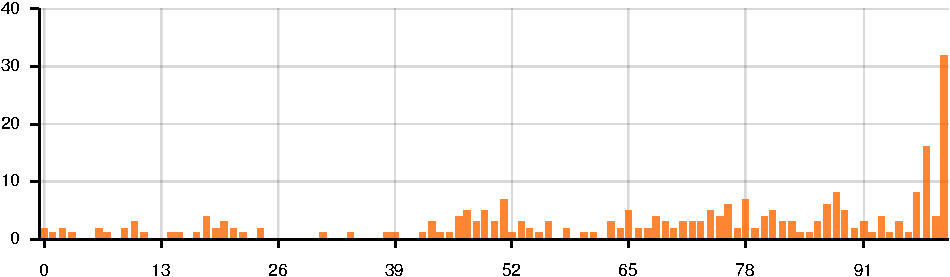
\includegraphics{figures/esurvey/c_com_u18_responsibility_companydev}}}
\caption{Auswertung Frage U18}
\label{U18}
\end{figure}

\subparagraph*{Frage: Daten auf Firmencomputer sind attraktiv für Aussenstehende}\mbox{}
\begin{figure}[H]
\centering
\framebox[\textwidth]{\scriptsize 0 = Trifft überhaupt nicht zu $\vert$ 100 = Trifft voll zu ($n: 255$, $\bar{x}: 43.15$, $\sigma: 35.28$)}
\framebox[\textwidth]{\scalebox{0.9}{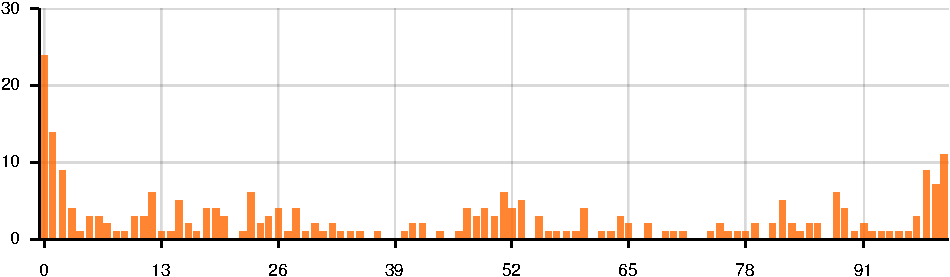
\includegraphics{figures/esurvey/c_com_u19_company_data}}}
\caption{Auswertung Frage U19}
\label{U19}
\end{figure}

\subparagraph*{Frage: Weiss, wie mit sensiblen Daten umgegangen werden muss}\mbox{}
\begin{figure}[H]
\centering
\framebox[\textwidth]{\scriptsize 0 = Trifft überhaupt nicht zu $\vert$ 100 = Trifft voll zu ($n: 255$, $\bar{x}: 78.96$, $\sigma: 20.19$)}
\framebox[\textwidth]{\scalebox{0.9}{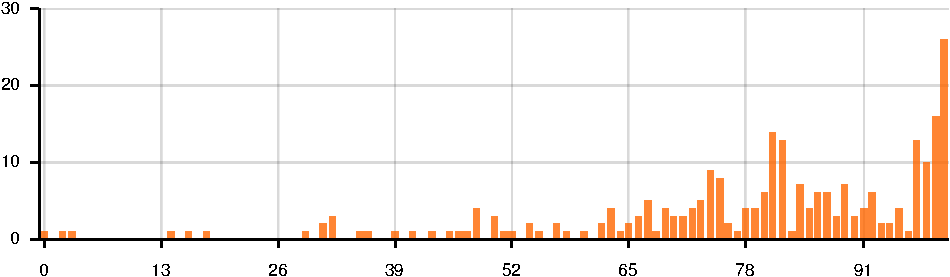
\includegraphics{figures/esurvey/c_com_u20_sensible_data}}}
\caption{Auswertung Frage U20}
\label{U20}
\end{figure}

\subparagraph*{Frage: Verwendung von Passwortmanager}\mbox{}
\begin{figure}[H]
\centering
\framebox[\textwidth]{\scriptsize $n: 255$}
\framebox[\textwidth]{\scalebox{0.9}{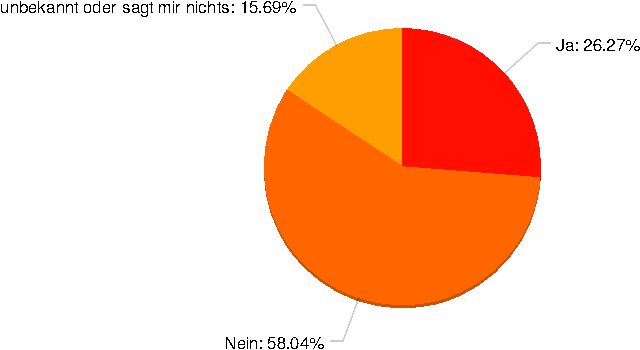
\includegraphics{figures/esurvey/c_com_u21_passwortmgr}}}
\caption{Auswertung Frage U21}
\label{U21}
\end{figure}

\subparagraph*{Frage: Email Attachement sind immer Virenfrei}\mbox{}
\begin{figure}[H]
\centering
\framebox[\textwidth]{\scriptsize $n: 255$}
\framebox[\textwidth]{\scalebox{0.9}{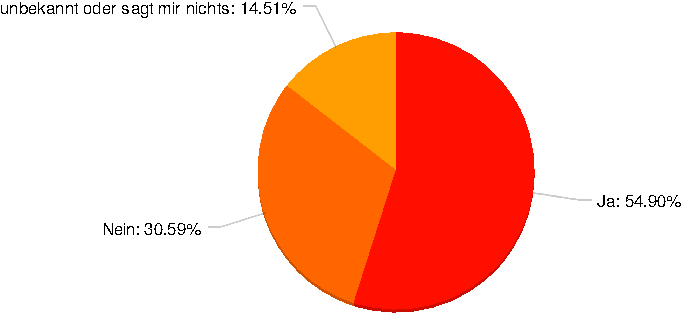
\includegraphics{figures/esurvey/c_com_u22_emailattachement}}}
\caption{Auswertung Frage U22}
\label{U22}
\end{figure}

\subparagraph*{Frage: Weitergabe Windows-Passwort an Arbeitskollegen}\mbox{}
\begin{figure}[H]
\centering
\framebox[\textwidth]{\scriptsize $n: 255$}
\framebox[\textwidth]{\scalebox{0.9}{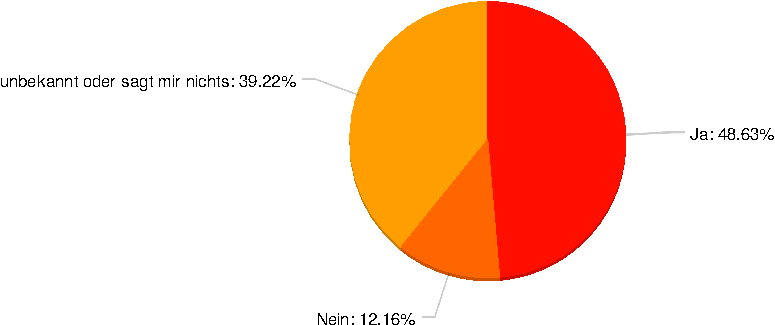
\includegraphics{figures/esurvey/c_com_u23_windows_pw}}}
\caption{Auswertung Frage U23}
\label{U23}
\end{figure}

\subparagraph*{Frage: Abgabe Zutrittsbadge an Arbeitskollegen}\mbox{}
\begin{figure}[H]
\centering
\framebox[\textwidth]{\scriptsize $n: 255$}
\framebox[\textwidth]{\scalebox{0.9}{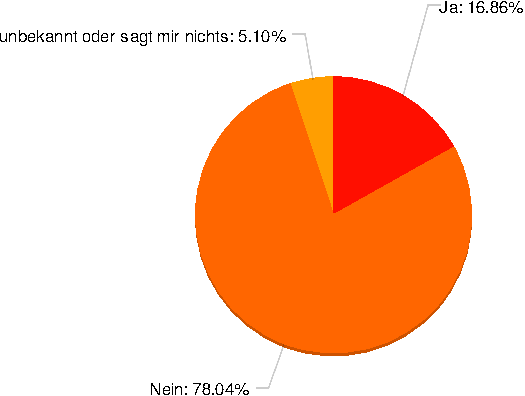
\includegraphics{figures/esurvey/c_com_u24_badgelending}}}
\caption{Auswertung Frage U24}
\label{U24}
\end{figure}

\subparagraph*{Frage: Sicherheitsvorfälle melden}\mbox{}
\begin{figure}[H]
\centering
\framebox[\textwidth]{\scriptsize $n: 255$}
\framebox[\textwidth]{\scalebox{0.9}{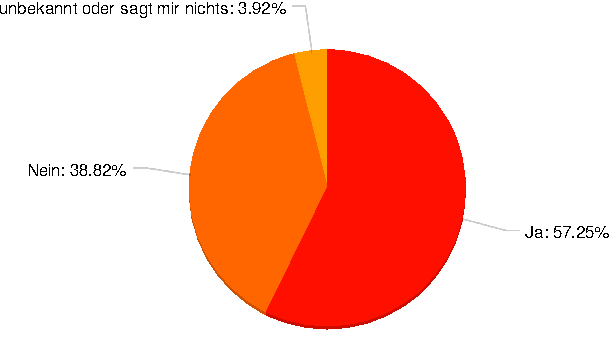
\includegraphics{figures/esurvey/c_com_u25_securityincident}}}
\caption{Auswertung Frage U25}
\label{U25}
\end{figure}

\subparagraph*{Frage: Bekanntheit Ansprechperson für Security Fragen}\mbox{}
\begin{figure}[H]
\centering
\framebox[\textwidth]{\scriptsize $n: 255$}
\framebox[\textwidth]{\scalebox{0.9}{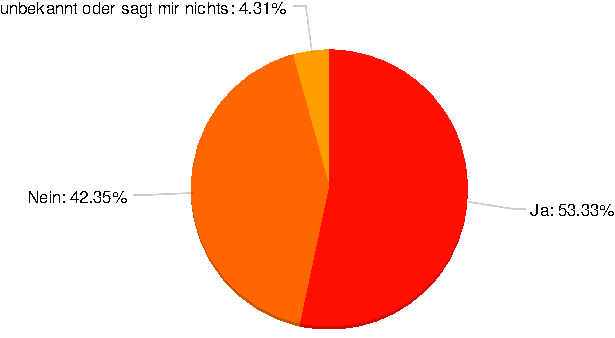
\includegraphics{figures/esurvey/c_com_u26_official_securityperson}}}
\caption{Auswertung Frage U26}
\label{U26}
\end{figure}

\end{document}